\documentclass[11pt, a4paper, twocolumn]{article}
\usepackage[a4paper,margin=1in,footskip=0.25in]{geometry}
 
\usepackage{graphicx}
\usepackage{enumerate}
\usepackage{amsmath}
\usepackage{amssymb}
\usepackage[utf8]{inputenc}
\usepackage{physics}
\usepackage{xcolor}
\usepackage{hyperref}
\usepackage{subfig}
\usepackage{floatrow}

\captionsetup[subfigure]{justification=raggedright}

\providecommand{\newoperator}[3]{%
	\newcommand*{#1}{\mathop{#2}#3}}
\providecommand{\renewoperator}[3]{%
	\renewcommand*{#1}{\mathop{#2}#3}}
	
\newoperator{\srot}%
	{\mathrm{rot}}{\nolimits}

\newoperator{\ent}%
	{\mathrm{ent}}{\nolimits}
	
\renewoperator{\Re}%
	{\mathrm{Re}}{\nolimits}
	
\renewoperator{\Im}%
	{\mathrm{Im}}{\nolimits}	
	
\makeatletter
\providecommand*{\diff}%
	{\@ifnextchar^{\DIfF}{\DIfF^{}}}
	
\def\DIfF^#1{%
	\mathop{\mathrm{\mathstrut d}}%
	\nolimits^{#1}\gobblespace}
	
\def\gobblespace{%
	\futurelet\diffarg\opspace}
	
\def\opspace{%
	\let\DiffSpace\!%
		\ifx\diffarg(%
			\let\DiffSpace\relax
		\else
			\ifx\diffarg[%
				\let\DiffSpace\relax
			\else
				\ifx\diffarg\{%
					\let\DiffSpace\relax
				\fi\fi\fi\DiffSpace}
				
\providecommand*{\deriv}[3][]{%
	\frac{\diff^{#1}#2}{\diff #3^{#1}}}
\providecommand*{\pderiv}[3][]{%
	\frac{\partial^{#1}#2}%
		{\partial #3^{#1}}}
		
\newcommand{\mean}[1]{\langle#1\rangle}

\begin{document}

\section{Bare}

\begin{figure}[h!]
	\includegraphics[width=\columnwidth]
	{../bin/figures/square/spc/Int64[].png}
	\caption{
		Interactions: ON
	}
\end{figure}

\begin{figure}[h!]
	\includegraphics[width=\columnwidth]
	{../bin/figures/square/spc_noint/Int64[].png}
	\caption{
		Interactions: OFF
	}
\end{figure}

\clearpage

\section{Single hop -- interacting}

\begin{figure}[h!]
	\includegraphics[width=\columnwidth]
	{../bin/figures/square/spc/[0].png}
	\caption{
		Interactions: ON
	}
\end{figure}

\begin{figure}[h!]
	\includegraphics[width=\columnwidth]
	{../bin/figures/square/spc/[1].png}
	\caption{
		Interactions: ON
	}
\end{figure}

\newpage

\section{Single hop -- non-interacting}

\begin{figure}[h!]
	\includegraphics[width=\columnwidth]
	{../bin/figures/square/spc_noint/[0].png}
	\caption{
		Interactions: OFF
	}
\end{figure}

\begin{figure}[h!]
	\includegraphics[width=\columnwidth]
	{../bin/figures/square/spc_noint/[1].png}
	\caption{
		Interactions: OFF
	}
\end{figure}

\clearpage

\section{Double hop -- interacting}

\begin{figure}[h!]
	\includegraphics[width=0.7\columnwidth]
	{../bin/figures/square/spc/[0, 0].png}
	\caption{
		Interactions: ON
	}
\end{figure}

\begin{figure}[h!]
	\includegraphics[width=0.7\columnwidth]
	{../bin/figures/square/spc/[0, 1].png}
	\caption{
		Interactions: ON
	}
\end{figure}

\begin{figure}[h!]
	\includegraphics[width=0.7\columnwidth]
	{../bin/figures/square/spc/[1, 0].png}
	\caption{
		Interactions: ON
	}
\end{figure}

\begin{figure}[h!]
	\includegraphics[width=0.7\columnwidth]
	{../bin/figures/square/spc/[1, 1].png}
	\caption{
		Interactions: ON
	}
\end{figure}

\section{Double hop -- non-inter}

\begin{figure}[h!]
	\includegraphics[width=0.7\columnwidth]
	{../bin/figures/square/spc_noint/[0, 0].png}
	\caption{
		Interactions: OFF
	}
\end{figure}

\begin{figure}[h!]
	\includegraphics[width=0.7\columnwidth]
	{../bin/figures/square/spc_noint/[0, 1].png}
	\caption{
		Interactions: OFF
	}
\end{figure}

\begin{figure}[h!]
	\includegraphics[width=0.7\columnwidth]
	{../bin/figures/square/spc_noint/[1, 0].png}
	\caption{
		Interactions: OFF
	}
\end{figure}

\begin{figure}[h!]
	\includegraphics[width=0.7\columnwidth]
	{../bin/figures/square/spc_noint/[1, 1].png}
	\caption{
		Interactions: OFF
	}
\end{figure}

\newpage

\section*{Acknowledgements}
We  kindly  acknowledge  support  by  the  (Polish)  National  Science  Centre  (NCN, Poland)  under  Projects  No. 2016/22/E/ST3/00560 (PW and KW), 2016/23/B/ST3/00839 (KW). The calculations were performed at the ICM cluster.


\end{document}